% !TeX program = xelatex
% !TeX TS-program = xelatex

\documentclass[aspectratio=169]{beamer}
\usepackage[main=russian,english]{babel}

\usepackage{pifont}
\newcommand{\cmark}{\ding{51}}
\newcommand{\xmark}{\ding{55}}

\usepackage{csquotes}

\newcommand{\myskip}{\vspace{\baselineskip}}

\setbeamertemplate{caption}[numbered]


\setbeamercolor{itemize item}{fg=black}
\setbeamercolor{itemize subitem}{fg=black}
\setbeamercolor{alerted text}{fg=black}
\setbeamertemplate{itemize items}{\textbullet}% отключает кошмарные синие треугольники
\setbeamerfont*{itemize/enumerate subbody}{parent=itemize/enumerate body}
\setbeamerfont*{itemize/enumerate subsubbody}{parent=itemize/enumerate subbody}
\setbeamerfont{alerted text}{series=\bfseries}


\title{Анализ ``мертвого'' кода}
\author{Команда ``Шерстяные волчары с мощными лапищами''}



\begin{document}

\begin{frame}
    \titlepage
\end{frame}

\begin{frame}{Немного о нас}
    \begin{figure}
        
\includegraphics[width=0.45\textwidth]{memes/volf.jpg}
        \caption{Про название}
    \end{figure}
\end{frame}

\begin{frame}{Немного о нас}
    Разрабатываем ПО ATMoSphere для устройств самообслуживания
    \begin{itemize}
        \item Много кода на C++
        \item Есть юнит-тесты
        \item Есть высокоуровневые тесты на бизнес-сценарии
    \end{itemize}
    \myskip
    \only<2>{Решили искать мёртвый код на примере нашей кодовой базы C++}
\end{frame}

\begin{frame}{``Мёртвый'' код}
    \begin{figure}
        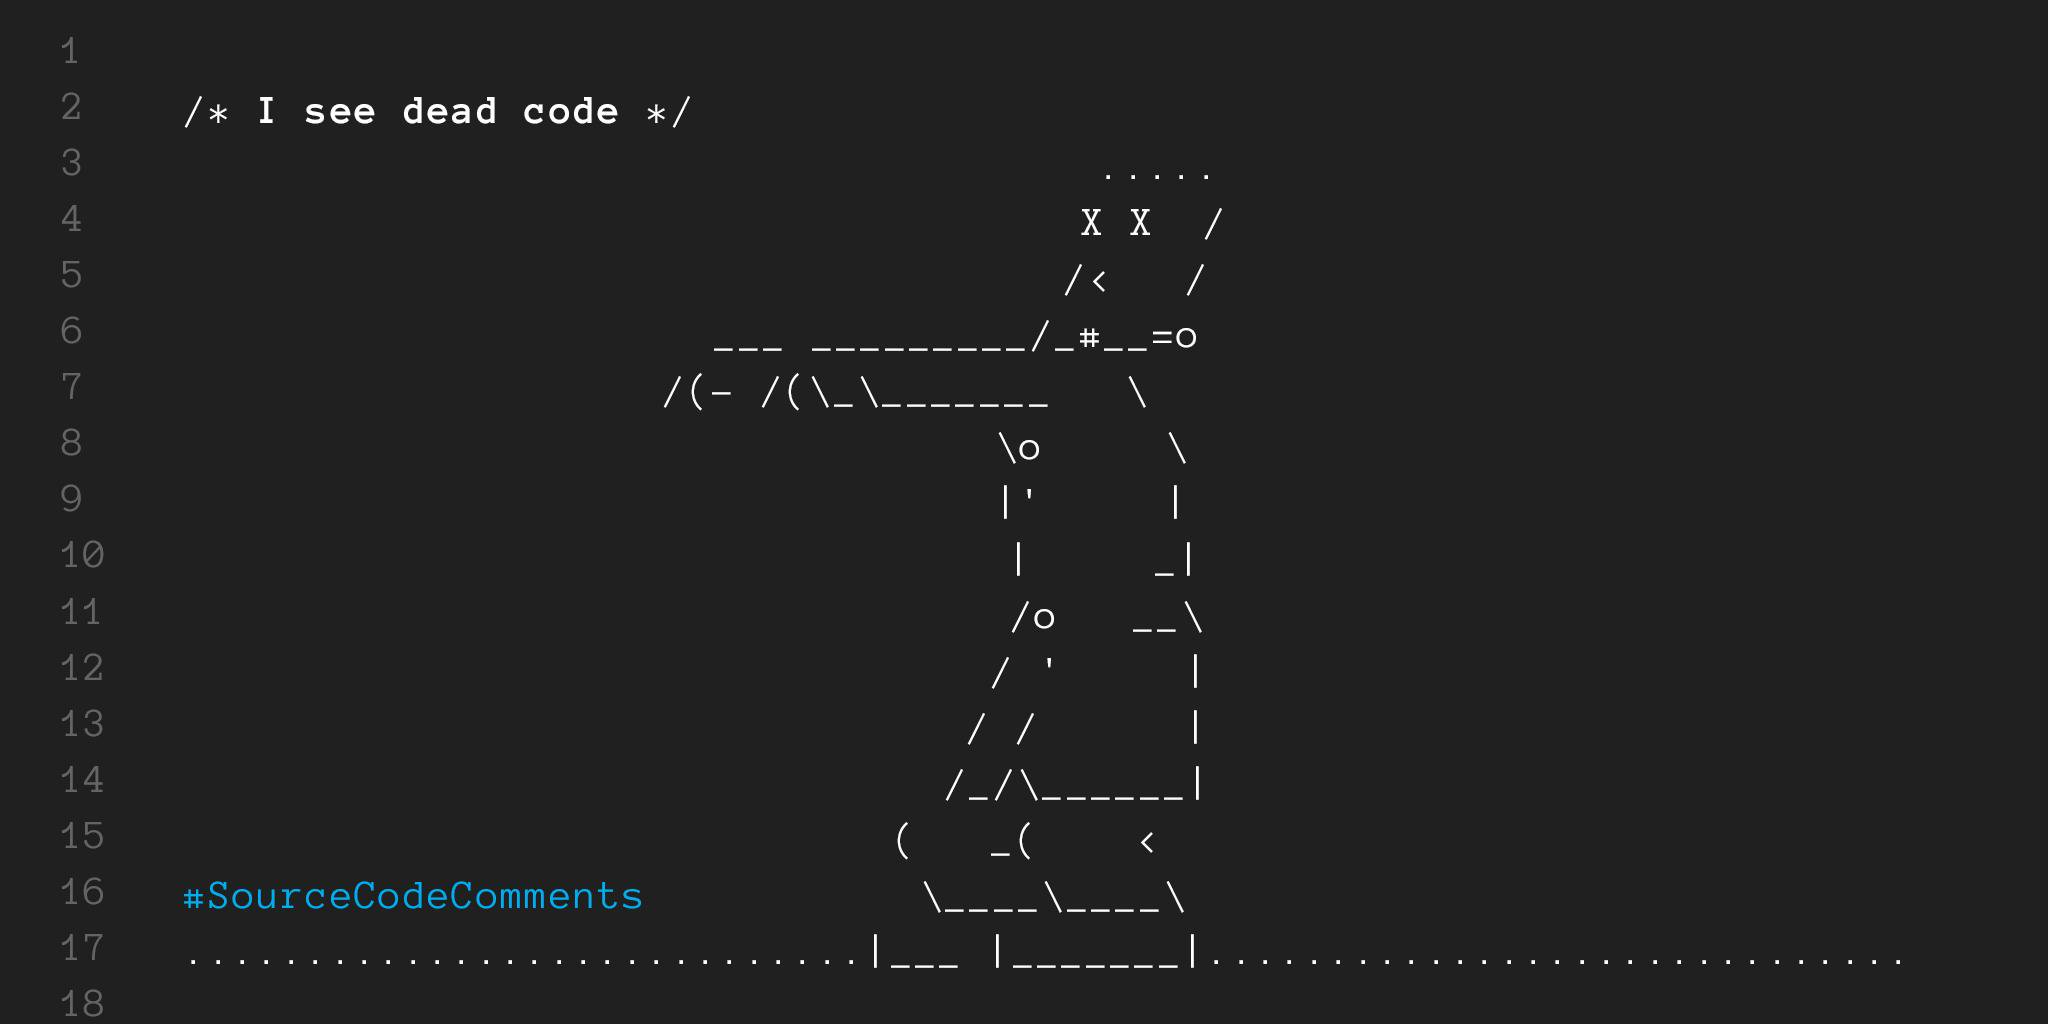
\includegraphics[width=0.9\textwidth]{memes/dead_code.jpg}
        \caption{Плавно переходим к теме кода}
    \end{figure}
\end{frame}

\begin{frame}{``Мёртвый'' код}
    Мёртвый код - это код, который не влияет на работу программы и может быть удалён.
\end{frame}

\begin{frame}{``Мёртвый'' код}
    \begin{figure}
        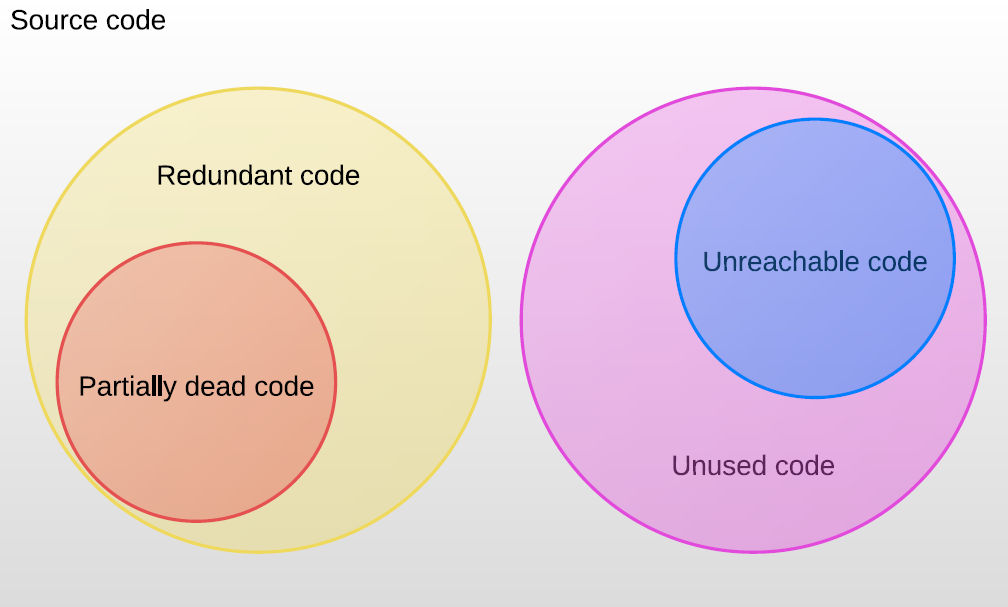
\includegraphics[width=0.75\textwidth]{memes/dead_code_scheme.jpg}
        \caption{Схемка из интернетов}
    \end{figure}
\end{frame}

\begin{frame}{``Мёртвый'' код}
    Разные синтаксические единицы
    \begin{itemize}
        \item Переменные
        \item Функции
        \item Классы
        \item Библиотеки
    \end{itemize}
\end{frame}

\begin{frame}{``Мёртвый'' код}
    Разные способы выявления
    \begin{itemize}
        \item Статический анализ
              \begin{itemize}
                  \item Флаги компилятора и линковщика
                  \item Анализаторы вроде CppCheck, Clang-Tidy, SonarCube, PvsStudio
                  \item Самостоятельный
              \end{itemize}
        \item Динамический анализ
              \begin{itemize}
                  \only<1>{\item Code coverage tool (например - gcovr)}
                        \only<2>{\item[\cmark] Code coverage tool (например - gcovr)}
              \end{itemize}
    \end{itemize}
\end{frame}

\begin{frame}{``Мёртвый'' код}
    \begin{figure}
        
\includegraphics[width=0.4\textwidth]{memes/finding_dead_code.png}
        \caption{Поиск мёртвого кода по версии ИИ}
    \end{figure}
\end{frame}

\begin{frame}{``Мёртвый'' код}
    Динамический анализ
    \begin{itemize}
        \item[\xmark] Синтаксические единицы
        \item[\cmark] Блоки кода
    \end{itemize}
\end{frame}

\begin{frame}{``Мёртвый'' код}
    Что ещё можно было бы искать
    \begin{itemize}
        \item ``Забытые''(не добавленные в cmake проект) файлы
        \item ``Забытые''(не влитые в develop/master) ветки в git
        \item Unreachable(недостижимый) код
    \end{itemize}
\end{frame}

\begin{frame}{``Мёртвый'' код}
    \begin{figure}
        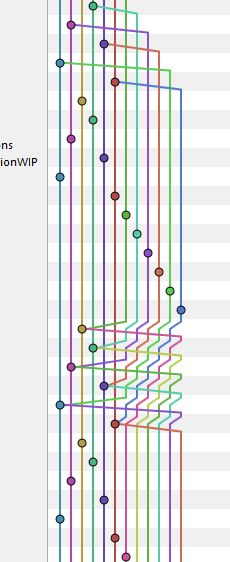
\includegraphics[width=0.18\textwidth]{memes/git.png}
        \caption{\textit{git}ar hero или мёртвые ветки в git}
    \end{figure}
\end{frame}

\begin{frame}{ Подготовка данных}
    \begin{itemize}
        \item Собираем репозиторий со специальным флагом сборки для coverage
        \item Запускаем тесты (желательно - тестирование бизнес-сценариев)
        \item Собираем данные по coverage - их мы и будем использовать в основе нашего анализа
    \end{itemize}
\end{frame}

\begin{frame}{Первичный анализ полученных данных}
    \begin{itemize}
        \item Считаем, что покрытый тестами код точно не является мёртвым
        \item Непокрытый код либо мёртвый, либо на него не написаны тесты
              \begin{itemize}
                  \item Такой подход заставляет писать больше высокоуровневых тестов
              \end{itemize}
        \item Дальше начинаем анализ не покрытых тестами блоков кода или файлов
    \end{itemize}
\end{frame}

\begin{frame}{Блоки кода vs файлы}
    Можно давать оценку ``мёртвости'' по файлам. Её легче получить, но она не слишком информативна. Это наш MVP1.

    \myskip
    Следующая итерация - это оценка для отдельных блоков кода(под блоками понимаются подряд идущие не покрытые тестами строки кода). Это наш MVP2.
\end{frame}


\begin{frame}{Система фильтров}
    Чтобы система получилась расширяемой, мы добавили фильтры, которые влияют на итоговую оценку
    \begin{itemize}
        \item Первый и основной фильтр - фильтр по данным от coverage
              \begin{itemize}
                  \item Для файлов смотрим процент непокрытых линий
                  \item Для блоков кода смотрим размер блока
              \end{itemize}
        \item Вторым мы выбрали фильтр по данным от git
              \begin{itemize}
                  \item Для файлов дату последней модификации и частоту модификаций
                  \item Для блоков кода смотрим среднее/крайнее значение последней модификации и частоту модификаций
              \end{itemize}
        \item Сюда же можно добавить какой-нибудь стат-анализ или любые другие метрики
    \end{itemize}
\end{frame}


\begin{frame}{Система фильтров}
    \begin{itemize}
        \item Фильтр для каждого блока/файла возвращает какую-то оценку ``в попугаях''
        \item Эти оценки умножаются на вес фильтра и затем суммируются
        \item Чем больше итоговое значение для файла/блока, тем больше вероятность того, что там есть мёртвый код
        \item Затем файлы/блоки кода сортируются на основе этой оценки
    \end{itemize}
\end{frame}

\begin{frame}{Заключение}
    \begin{center}
        Работает - не трогай!

        Не работает? Это MVP...
    \end{center}
\end{frame}



\end{document}